\chapter[Optimized partitioning for SMR]{Optimized partitioning for SMR}
\label{sec:dynastar}

% \section{Decentralize partitioning is inefficient}

\dssmr{} addresses the limitations of \ssmr{} by adapting the partitioning
scheme as workloads change, by moving data ``on demand'' to maximize the number
of single partition user commands, while avoiding imbalances in the load of the
partitions. The major challenge in this approach is determining how the system
selects the partition to which to move data. \dssmr{} selects partitions
randomly, which allows for a completely decentralized implementation, in which
partitions make only local choices about data movement. We refer to this
approach as \emph{decentralized partitioning}. This approach works well for data
with \emph{strong locality}, but it is unstable for workloads with \emph{weak
locality}\footnote{Workloads are refered as \emph{strong locality} if that can
be partitioned in a way that would both (i) allow commands to be executed at a
single partition only, and (ii) evenly distribute data so that load is balanced
among partitions. Conversely, workloads that cannot avoid multi-partition
commands with balanced load among partitions exhibit \emph{weak locality}.}.
This happens because with weak locality, objects in \dssmr{} are constantly
being moved back and forth between partitions without converging to a stable
configuration.
% Figure~\ref{fig:dynastar-motivation} shows the result of our motivating
% experiment that compares two. In the experiment, we measured the throughput
% and number of state moves over time with two different workloads: one with
% strong locality and one with weak locality. The workloads are inspired by the
% social network Twitter, in which the network is modeled as a graph, and users
% can “post” messages. The social graph was generated using a Zipfian
% distribution, where the Zipf parameter was adjusted to alter the locality. For
% brevity, we postpone the details of the experimental setup until
% Section~\ref{sec:experiments}. As Figure~\ref{fig:dynastar-motivation} shows,
% the decentralized dynamic approach works well for data with strong locality,
% but is unstable for workloads with weak locality, since data is constantly
% moved from one partition to another.

In this chapter, we introduce \dynastar, a new dynamic approach to the state
partitioning problem. Like the other dynamic approach, \dynastar does not
require any a priori knowledge about the workload. However, \dynastar differs
from the prior approach because it maintains a location oracle with a global
view of the application state. The oracle minimizes the number of state
relocations by monitoring the workload, and re-computing an optimized
partitioning on demand using a static partitioning algorithm.

% \begin{figure*}[ht!] \centering \begin{subfigure}[b]{0.45\textwidth}
%   \centering
%   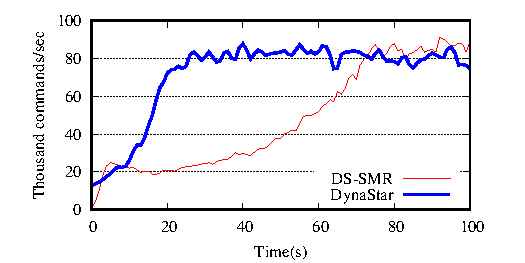
\includegraphics[width=0.95\columnwidth]{figures/dynastar_experiment/proposal-tp-strong-locality}
%   \caption{Throughput with strong locality} \end{subfigure}
%   \begin{subfigure}[b]{0.45\textwidth} \centering
%   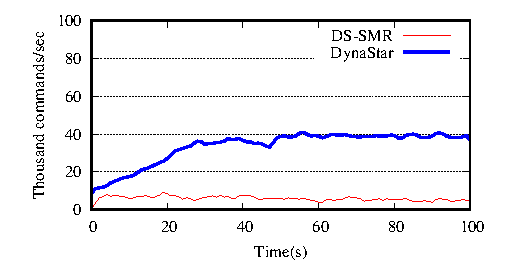
\includegraphics[width=0.95\columnwidth]{figures/dynastar_experiment/proposal-tp-weak-locality}
%   \caption{Throughput with weak locality} \end{subfigure} \\
%   \begin{subfigure}[b]{0.45\textwidth} \centering
%     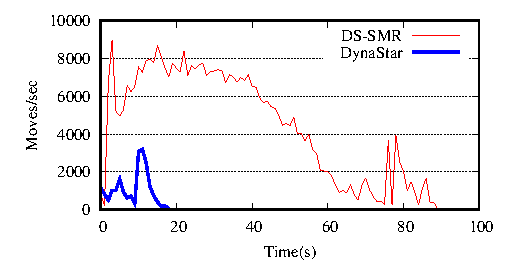
\includegraphics[width=0.95\columnwidth]{figures/dynastar_experiment/proposal-moves-strong-locality}
%     \caption{Number of move commands with strong locality} \end{subfigure}
%     \begin{subfigure}[b]{0.45\textwidth} \centering
%     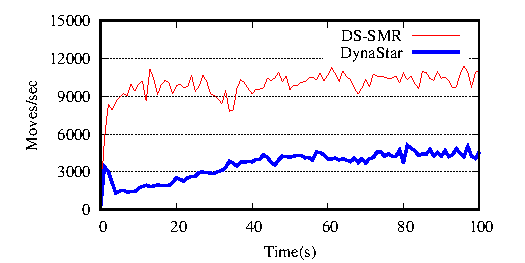
\includegraphics[width=0.95\columnwidth]{figures/dynastar_experiment/proposal-moves-weak-locality}
%     \caption{Number of move commands with weak locality} \end{subfigure}
%     \caption{\dynastar and DS-SMR under strong and weak locality, 4
%     partitions.} \label{fig:dynastar-motivation} \end{figure*}


\section{\dynastar: Optimized dynamic partitioning for SMR}
\label{sec:dynastaridea}

The key insights of \dynastar are to create the workload graph on-the-fly and
use graph partitioning techniques to efficiently relocate application state
on-demand.
\begin{itemize}
\item \emph{On-the-fly workload modeling.}
\dynastar models a service workload as a graph $G = (V, E)$, where vertices
represent state variables and edges dependencies between variables. An edge
connects two variables in the graph if a command accesses both of them. A
location oracle builds the workload graph based on feedback from the clients or
partitions, as commands are executed.
\item \emph{On-demand relocation of service state.}
Periodically, the oracle computes a partitioning of the workload graph. Based on
this partitioning and the current location of variables, the oracle determines
the destination partition for commands that access variables spread on multiple
partitions. When computing the destination partition, the oracle strives to
minimize the number of moves. Variables are moved on demand, when a command
needs the variables.
\end{itemize}

In \dynastar a move request is multicast together with the command that
triggered the request.
%a partition executes a command right after it has gathered all variables it
%needs.
Therefore, differently from DS-SMR, \dynastar ensures termination without
resorting to expensive mechanisms (i.e., S-SMR).


\subsection{The \dynastar protocol}
\setcounter{secnumdepth}{3}
Sections~\ref{sec:dynastar-client}, \ref{sec:dynastar-server}, and
\ref{sec:dynastar-oracle} describe the client, server and oracle processes,
respectively. For brevity, we omit the delete command since the coordination
involved in the create and delete commands are analogous. The oracle is
replicated and handled as a partition. In the discussion in this section, every
command involves the oracle. In the next section, we explain how clients can use
a cache to avoid the oracle in the execution of most commands.

\subsubsection{The client process}
\label{sec:dynastar-client}
To execute a command, the client atomically multicasts the command to the
oracle. The oracle replies with a prophecy, which may already tell the client
that the command cannot be executed (e.g., it needs a variable that does not
exist, it tries to create a variable that already exists). If the command can be
executed, the client receives a prophecy containing the partition where the
command will be executed. The client then waits for the result of the execution
of the command.
% The client must retry the command if the partition cannot execute the command.
% This happens if some of the variables needed by the command were moved to
% another partition due to other commands. To ensure that a command is
% eventually executed, after retrying a few times, the client falls back to
% using \ssmr{}, multicasting the command to all partitions (and the oracle, in
% case of a create or delete command).

\subsubsection{The server process}
\label{sec:dynastar-server}
When a server delivers a command $C$, multicast by the oracle, it executes the
command and sends the response back to the client. If not all the variables
needed by the command are in a single partition, the oracle issues a move
command that involves all partitions containing the needed variables.
%If one or more variables are not stored in a single partition, the server
%returns a message to the client to retry the operation. This happens if the
%oracle moved some variables to another partition as part of another command.
In this case, a server in the source partitions reliably multicasts all the
needed variables stored locally to the destination partition. Servers in the
destination partition wait for a message from each source partition. Once all
variables needed are available, destination servers execute the command $C$ and
send the response back to the client.

%When a server delivers a message to create a variable (and similarly to delete
%an existing variable), it coordinates with the oracle (Task 3). The exchange of
%signals between the partition where the variable will be created and the oracle
%ensures that interleaved executions between create and delete commands will not
%lead to violations of linearizability (i.e., this is essentially the execution
%of a multi-partition command involving the oracle and a
%partition~\cite{bezerra2014ssmr}).



\subsubsection{The oracle}
\label{sec:dynastar-oracle}
When the oracle delivers a request, it distinguishes between two cases.
\begin{itemize}
\item If the command is to create a variable $v$, and $v$ does not already
exist, the oracle chooses a random partition for $v$, multicasts the create
command to the partition and itself, and returns the partition to the client as
a prophecy (Figure~\ref{fig:oracle_repartition}).
\item If the command reads and writes existing variables, the oracle first
checks that all such variables exist. If the variables exist and they are all in
a single partition, the oracle multicasts the command to that partition for
execution. If the variables are distributed in multiple partitions, the oracle
determines the destination partition, and atomically multicasts a command to the
involved partitions and to itself so that all variables are moved to the
destination partition. The destination partition executes the command once it
has received all variables needed by the command.
%In either case, oracle returns a prophecy back to the client with the
%destination partition.
\end{itemize}

% \input{dynastar_algorithm_client_proxy}
% \input{dynastar_algorithm_server_proxy}
% \input{dynastar_algorithm_oracle_proxy}

\begin{figure*}
\begin{minipage}[b]{1\linewidth} % A minipage that covers the whole width of the
page
\centering
      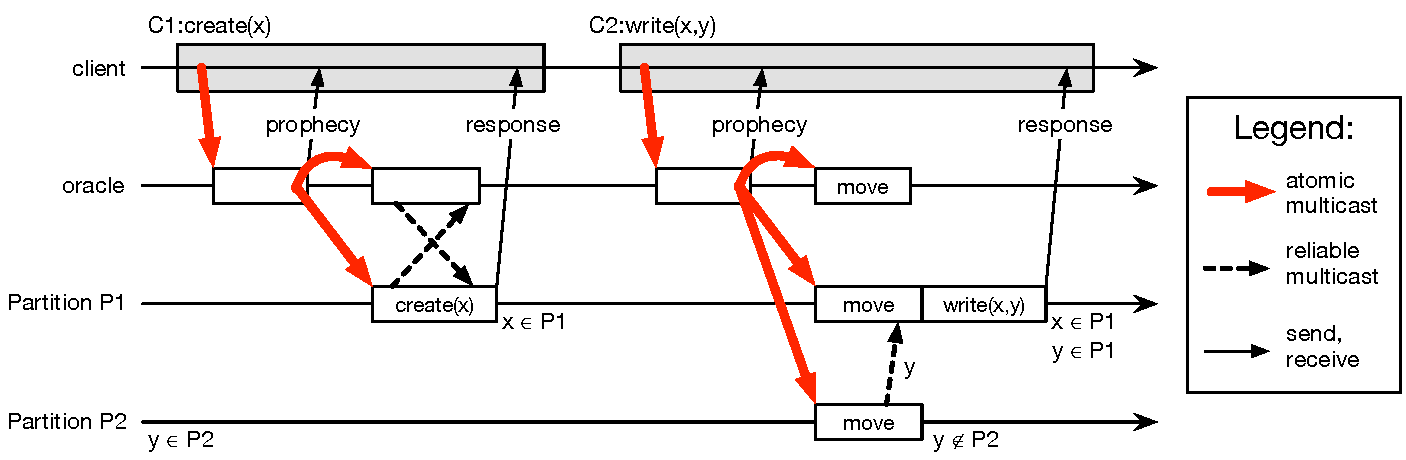
\includegraphics[width=0.9\linewidth]{figures/dynastar}
\end{minipage}
\caption{The execution of a create command and a write command in \dynastar.}
\label{fig:oracle_repartition}
\end{figure*}

Upon delivering a create or a move command, the oracle updates its partition
information. As part of a create command, the oracle coordinates with the
partition to ensure correctness~\cite{bezerra2014ssmr}.
%
The oracle also keeps track of the workload graph, computes a partitioning of
the graph, and determines the destination partition for move operations. To
maintain the workload graph, the oracle receives hints with variables (i.e.,
vertices in the graph) and executed commands (i.e., edges in the graph). These
hints can be submitted by the clients or by the partitions, which collect data
upon executing commands and periodically inform the oracle.

To compute an optimized partitioning, the oracle uses a graph partitioner. A new
partitioning can be requested by the application, by a partition, or by the
oracle itself (e.g., upon delivering a certain number of hints). To determine
the destination partition of a set of variables, as part of a move, the oracle
uses
% the current location of variables and
the last computed partitioning.


\subsection{Performance optimizations}
%\subsection{Performance optimizations}
\label{sec:optm}

In the algorithm presented in the previous section, clients always need to
involve the oracle, and the oracle dispatches every command to the partitions
for execution. Obviously, if every command involves the oracle, the system is
unlikely to scale, as the oracle will likely become a bottleneck. To address
this issue, clients are equipped with a location cache. Before submitting a
command to the oracle, the client checks its location cache. If the cache
contains the partition of the variables needed by the command and all variables
are in a single destination partition, the client can atomically multicast the
command to the partition and avoid contacting the oracle.

The client still needs to contact the oracle in one of these situations:
(a)~according to the client's cache, not all variables accessed by the command
are in the same partition and it is necessary to move variables; (b)~the cache
contains outdated information, and the command is multicast to a partition that
does not contain all needed variables; or (c)~the command is a create, in which
case it must involve the oracle, as explained before. If the cache contains
outdated information and the addressed partition does not contain all the
variables accessed by the command, the partition tells the client to retry the
command. In this case, the client contacts the oracle and then updates its cache
with the oracle's response.
